%
% hardware.tex
%
% Copyright (C) 2019 by Universidade Federal de Santa Catarina.
%
% OBDH 2.0 Documentation
%
% This work is licensed under the Creative Commons Attribution-ShareAlike 4.0
% International License. To view a copy of this license,
% visit http://creativecommons.org/licenses/by-sa/4.0/.
%

%
% \brief Hardware chapter.
%
% \author Gabriel Mariano Marcelino <gabriel.mm8@gmail.com>
%
% \institution Universidade Federal de Santa Catarina (UFSC)
%
% \version 0.1.0
%
% \date 20/10/2019
%

\chapter{Hardware} \label{ch:hardware}

\section{Interfaces}

\begin{figure}[!ht]
    \begin{center}
        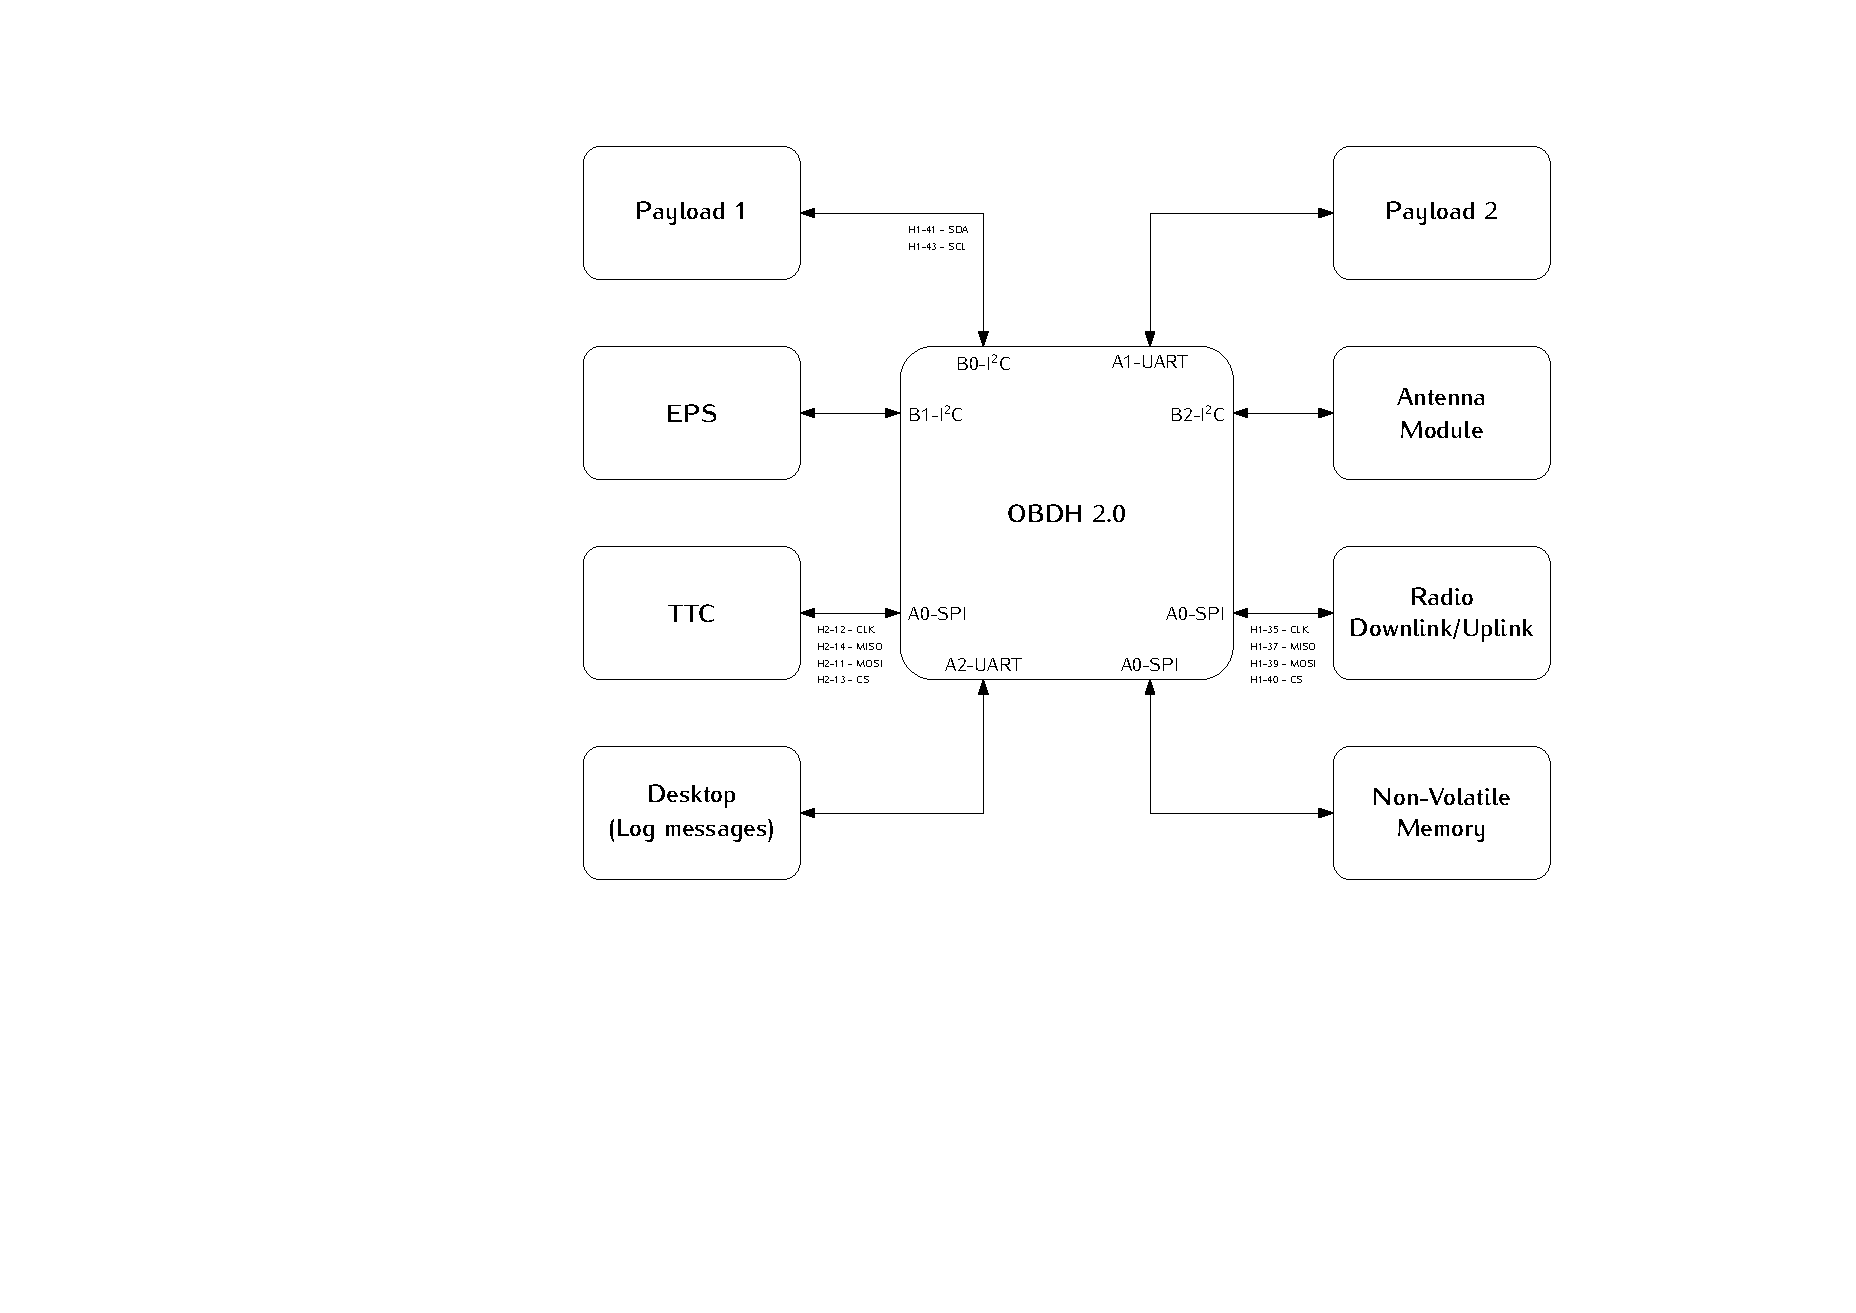
\includegraphics[width=\textwidth]{figures/diagram_interfaces.pdf}
        \caption{Interfaces diagram.}
        \label{fig:diagram-interfaces}
    \end{center}
\end{figure}

Currently, ``\textit{Payload 1}'' and ``\textit{Payload 2}'' are ``\textit{Payload-X}'' and ``\textit{Payload EDC}'' respectively.

\section{External Connectors}

\subsection{PC-104}

\begin{table}[!h]
    \centering
    \begin{tabular}{cllll}
        \toprule[1.5pt]
        \textit{Pin [A-B]} & \textit{H1A}     & \textit{H1B}     & \textit{H2A}  & \textit{H2B}  \\
        \midrule
        1-2                & -                & -                & -             & -             \\
        3-4                & -                & -                & -             & -             \\
        5-6                & GPIO\_0          & GPIO\_1          & -             & -             \\
        7-8                & GPIO\_2          & GPIO\_3          & -             & -             \\
        9-10               & GPIO\_4          & -                & -             & -             \\
        11-12              & GPIO\_5          & GPIO\_6          & SPI\_0\_MOSI  & SPI\_0\_CLK   \\
        13-14              & GPIO\_7          & -                & SPI\_0\_CS\_1 & SPI\_0\_MISO  \\
        15-16              & -                & -                & -             & -             \\
        17-18              & -                & GPIO\_8          & -             & -             \\
        19-20              & -                & GPIO\_9          & -             & -             \\
        21-22              & -                & -                & -             & -             \\
        23-24              & -                & -                & -             & -             \\
        25-26              & RS485\_TX+       & RS485\_TX-       & -             & -             \\
        27-28              & RS485\_RX+       & RS485\_RX-       & -             & -             \\
        29-30              & GND              & GND              & GND           & GND           \\
        31-32              & GND              & GND              & GND           & GND           \\
        33-34              & -                & -                & -             & -             \\
        35-36              & SPI\_0\_CLK      & -                & VCC\_3V3\_ANT & VCC\_3V3\_ANT \\
        37-38              & SPI\_0\_MISO     & -                & -             & -             \\
        39-40              & SPI\_0\_MOSI     & SPI\_0\_CS\_0    & -             & -             \\
        41-42              & I2C\_0\_SDA      & -                & -             & -             \\
        43-44              & I2C\_0\_SCL      & -                & -             & -             \\
        45-46              & VCC\_3V3         & VCC\_3V3         & VCC\_BAT      & VCC\_BAT      \\
        47-48              & -                & -                & -             & -             \\
        49-50              & -                & -                & -             & -             \\
        51-52              & -                & -                & -             & -             \\
        \bottomrule[1.5pt]
    \end{tabular}
    \caption{PC-104 connector pinout.}
    \label{tab:pc104-pins}
\end{table}

\subsection{Antenna Module}



\subsection{Programmer}



\subsection{Debug Interface}



\subsection{Daughterboard}

The daughterboard interface uses the Samtec FSI-110-D connector. An illustration of the connector can be seen in the \autoref{fig:samtec-connector}.

\begin{figure}[!ht]
    \begin{center}
        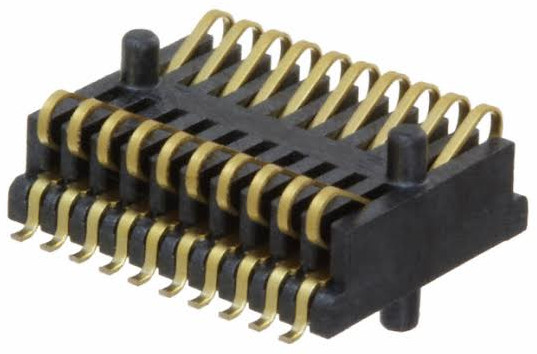
\includegraphics[width=0.4\textwidth]{figures/samtec_fsi-110-03-g-d-ad.jpeg}
        \caption{Samtec FSI-110-03-G-D-AD connector.}
        \label{fig:samtec-connector}
    \end{center}
\end{figure}

The pinout of the daughterboard interface are available in the \autoref{tab:daugtherboard-connector-pins}.

\begin{table}[!h]
    \centering
    \begin{tabular}{cllll}
        \toprule[1.5pt]
        \textit{Pin [A-B]} & \textit{Row A} & \textit{Row B} \\
        \midrule
        1-2                & VCC\_3V3       & GND            \\
        3-4                & VCC\_3V3\_ANT  & GND            \\
        5-6                & VCC\_BAT       & GND            \\
        7-8                & GPIO\_0        & GPIO\_1        \\
        9-10               & GPIO\_2        & GPIO\_3        \\
        11-12              & SPI\_0\_CLK    & ADC\_0         \\
        13-14              & SPI\_0\_MISO   & ADC\_1         \\
        15-16              & SPI\_0\_MOSI   & ADC\_2         \\
        17-18              & SPI\_0\_CS\_0  & I2C\_2\_SDA    \\
        19-20              & SPI\_0\_CS\_1  & I2C\_2\_SCL    \\
        \bottomrule[1.5pt]
    \end{tabular}
    \caption{Daughterboard connector pinout.}
    \label{tab:daugtherboard-connector-pins}
\end{table}

\subsubsection{Guidelines}

The recommended shape and size of the daughterboard can be seen in the \autoref{fig:daughterboard-size}.

\begin{figure}[!ht]
    \begin{center}
        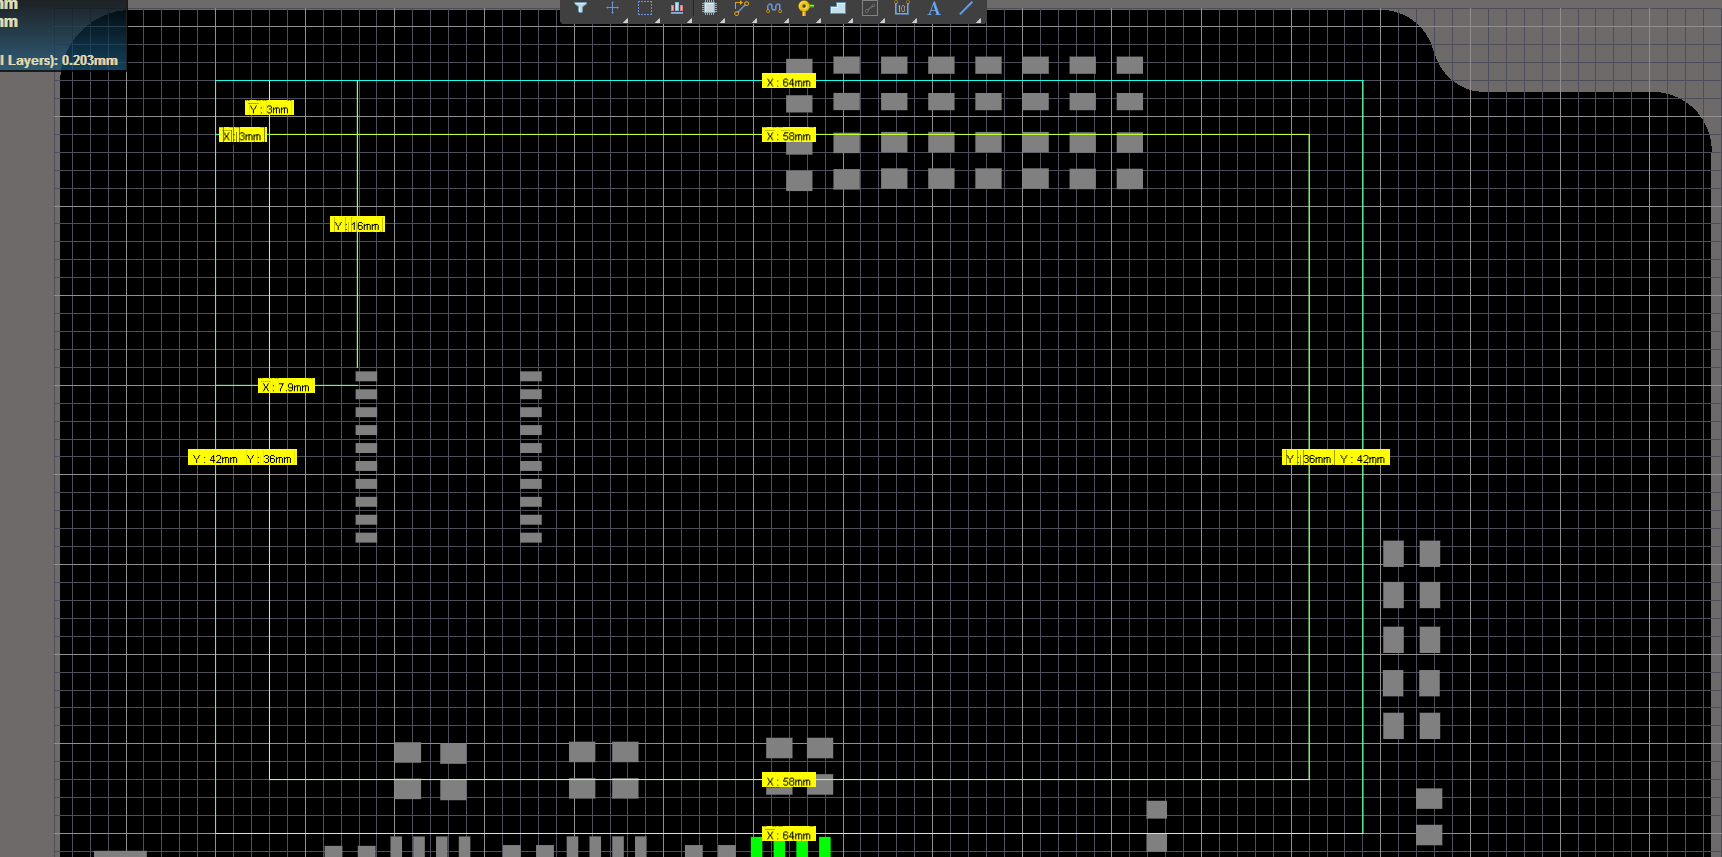
\includegraphics[width=\textwidth]{figures/daughterboard_size.png}
        \caption{Recommended shape and size of the daughterboard.}
        \label{fig:daughterboard-size}
    \end{center}
\end{figure}

\section{Microcontroller}

MSP430F6659.

\subsection{Pinout}

\begin{table}[!h]
    \centering
    \begin{tabular}{lcl}
        \toprule[1.5pt]
        \textit{Pin Code} & \textit{Pin Number} & \textit{Signal}       \\
        \midrule
        P1.0              & 34                  & MAIN\_RADIO\_ENABLE   \\
        P1.1              & 35                  & MAIN\_RADIO\_GPIO0    \\
        P1.2              & 36                  & MAIN\_RADIO\_GPIO1    \\
        P1.3              & 37                  & MAIN\_RADIO\_GPIO2    \\
        P1.4              & 38                  & MAIN\_RADIO\_RESET    \\
        P1.5              & 39                  & MAIN\_RADIO\_SPI\_CS  \\
        P1.6              & 40                  & TTC\_MCU\_SPI\_CS     \\
        P1.7              & 41                  & -                     \\
        \midrule
        P2.0              & 17                  & SPI\_CLK              \\
        P2.1              & 18                  & I2C0\_SDA             \\
        P2.2              & 19                  & I2C0\_SCL             \\
        P2.3              & 20                  & -                     \\
        P2.4              & 21                  & SPI\_MOSI             \\
        P2.5              & 22                  & SPI\_MISO             \\
        P2.6              & 23                  & -                     \\
        P2.7              & 24                  & -                     \\
        \midrule
        P3.0              & 42                  & I2C0\_EN              \\
        P3.1              & 43                  & I2C1\_EN              \\
        P3.2              & 44                  & I2C2\_EN              \\
        P3.3              & 45                  & I2C0\_READY           \\
        P3.4              & 46                  & I2C1\_READY           \\
        P3.5              & 47                  & I2C2\_READY           \\
        P3.6              & 48                  & PC104\_GPIO0          \\
        P3.7              & 49                  & PC104\_GPIO1          \\
        \midrule
        P4.0              & 50                  & PC104\_GPIO2          \\
        P4.1              & 51                  & PC104\_GPIO3          \\
        P4.2              & 52                  & MEM\_HOLD             \\
        P4.3              & 53                  & MEM\_RESET            \\
        P4.4              & 54                  & MEM\_SPI\_CS          \\
        P4.5              & 55                  & -                     \\
        P4.6              & 56                  & -                     \\
        P4.7              & 57                  & -                     \\
        \midrule
        P5.0              & 9                   & VREF                  \\
        P5.1              & 10                  & AGND                  \\
        P5.2              & 28                  & SYSTEM\_FAULT\_LED    \\
        P5.3              & 31                  & SYSTEM\_LED           \\
        P5.4              & 32                  & PAYLOAD\_0\_ENABLE    \\
        P5.5              & 33                  & PAYLOAD\_1\_ENABLE    \\
        P5.6              & 16                  & -                     \\
        P5.7              & 88                  & -                     \\
        \midrule
        P6.0              & 97                  & D\_BOARD\_ADC0        \\
        P6.1              & 98                  & D\_BOARD\_ADC1        \\
        P6.2              & 99                  & D\_BOARD\_ADC2        \\
        P6.3              & 100                 & OBDH\_CURRENT\_ADC    \\
        P6.4              & 1                   & OBDH\_VOLTAGE\_ADC    \\
        P6.5              & 2                   & D\_BOARD\_SPI\_CS0    \\
        P6.6              & 3                   & D\_BOARD\_SPI\_CS1    \\
        P6.7              & 4                   & -                     \\
        \midrule
        P7.0              & -                   & -                     \\
        P7.1              & -                   & -                     \\
        P7.2              & 84                  & XT2\_N                \\
        P7.3              & 85                  & XT2\_P                \\
        P7.4              & 5                   & D\_BOARD\_GPIO0       \\
        P7.5              & 6                   & D\_BOARD\_GPIO1       \\
        P7.6              & 7                   & D\_BOARD\_GPIO2       \\
        P7.7              & 8                   & D\_BOARD\_GPIO3       \\
        \midrule
        P8.0              & 58                  & -                     \\
        P8.1              & 59                  & -                     \\
        P8.2              & 60                  & UART1\_TX             \\
        P8.3              & 61                  & UART1\_RX             \\
        P8.4              & 62                  & -                     \\
        P8.5              & 65                  & I2C1\_SDA             \\
        P8.6              & 66                  & I2C1\_SCL             \\
        P8.7              & 67                  & ANTENNA\_GPIO         \\
        \midrule
        P9.0              & 68                  & -                     \\
        P9.1              & 69                  & -                     \\
        P9.2              & 70                  & UART0\_TX             \\
        P9.3              & 71                  & UART0\_RX             \\
        P9.4              & 72                  & WDI\_EXT              \\
        P9.5              & 73                  & I2C2\_SDA             \\
        P9.6              & 74                  & I2C2\_SCL             \\
        P9.7              & 75                  & MR\_WDOG              \\
        \midrule
        PJ.0              & 92                  & TP21                  \\
        PJ.1              & 93                  & TP22                  \\
        PJ.2              & 94                  & TP23                  \\
        PJ.3              & 95                  & TP24                  \\
        \midrule
        -                 & 13                  & XT1IN                 \\
        -                 & 14                  & XT1OUT                \\
        -                 & 96                  & JTAG\_TDO\_TDI        \\
        -                 & 91                  & JTAG\_TCK             \\
        \bottomrule[1.5pt]
    \end{tabular}
    \caption{Microcontroller pinout.}
    \label{tab:mcu-pinout}
\end{table}

\section{External Watchdog}

Additionally to the internal watchdog timer of the microcontroller, to ensure a system reset in case of a software freeze, an external watchdog circuit is being used. For that, the TPS3823 IC from Texas Instruments was chosen. This IC is a voltage monitor with a watchdog timer circuit.

This circuit works this way: if the WDI pin remains high or low longer than the timeout period, then reset is triggered. The timer clears when reset is asserted or when WDI sees a rising edge or a falling edge.

The watchdog timer task clears the TPS3823 timer by toggling the WDI pin at every 100 ms. If the WDI pin state stays unmodified for more than 1600 ms, the reset pin is cleared and the microcontroller is reseted.

This circuit can be seen in the \autoref{fig:ext-wdt-circuit}.

\begin{figure}[!ht]
    \begin{center}
        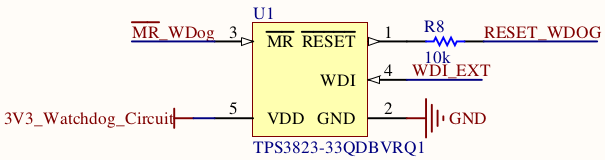
\includegraphics[width=0.75\textwidth]{figures/ext-watchdog-circuit.png}
        \caption{External watchdog timer circuit.}
        \label{fig:ext-wdt-circuit}
    \end{center}
\end{figure}

\section{Non-Volatile Memory}

The non-volatile memory is composed by a NOR flash memory with 1 Gb of capacity (or 128 MB). The used model is the Micron MT25QL01GBBB.

As can be seen in \autoref{fig:diagram-interfaces}, a SPI bus is used to communicate with this peripheral.
